\documentclass{customStyle}

%% ---- Additional packages (add as needed) ----
\usepackage{booktabs}      	% Professional tables (\toprule, \midrule, \bottomrule)
\usepackage{multirow}      	% Multi-row table cells
%% graphicx, amsmath cls tarafından zaten yuklendiginden tekrar eklenmez.
%% amssymb da eklenmez -- newtxmath ile \Bbbk catismasi yaratir.
\usepackage{subcaption}    % Sub-figures (optional)
\usepackage{hyperref}      % Clickable links in PDF (load last)
\usepackage[polish]{babel}
\usepackage{float}
\hypersetup{
  colorlinks = true,
  linkcolor  = black,
  citecolor  = black,
  urlcolor   = black
}

%% ============================================================
%%  TITLE BLOCK INFORMATION
%% ============================================================

\title{Klasyfikacja meczów League of Legends przy ograniczonych danych z pierwszych 10 minut meczu}

%% Authors: use \textsuperscript{*} for affiliation markers
%% \orcidlink{xxxx-xxxx-xxxx-xxxx} : yazar adının hemen yanına ORCID iD ikonu ekler.
%% İkon tıklanabilir olup https://orcid.org/xxxx-xxxx-xxxx-xxxx adresine yönlendirir.
%% ORCID ID'si olmayan yazar için \orcidlink{} satırını kaldırın.
\author{%
  Michał Wojda\textsuperscript{*} {\small (227753)} ,
  Sebastian Śmietański\textsuperscript{*} {\small (227914)}, \\
  Tomasz Teofilak\textsuperscript{*} {\small (227674)},
  Tomasz Żołądek\textsuperscript{*} {\small (230998)}%
}

%% Affiliations (one line per group, separated by \\)
\ijaffiliation{%
  \textsuperscript{*}Wydział Zastosowań Informatyki i Matematyki, Szkoła Główna Gospodarstwa Wiejskiego, 	Warszawa, Polska
}

%% E-mail addresses of all authors (in parentheses, comma-separated)
\ijemail{%
  s227753@sggw.edu.pl,
  s227914@sggw.edu.pl,
  s227674@sggw.edu.pl,
  s230998@sggw.edu.pl%
}

\receivedaccepted{09.06.2026}{09.06.2027}

%% ============================================================
%%  RUNNING HEADER METADATA
%%  Bu bilgiler her sayfanın üst bilgisinde görünür.
%% ============================================================

%% Kısa yazar listesi: "Soyad et al." veya iki yazar ise "Soyad1 and Soyad2"
\ijshortauthor{F.~Author et al.}

%% Dergi cilt, sayı, ay ve yıl bilgisi (editörlük tarafından doldurulur)
\ijvolume{x}
\ijissue{x}
\ijpubmonth{Month}
\ijpubyear{xxxx}

%% Makale türü: "Research Article" veya "Review Article"
\ijarticletype{Metody Analizy Danych, Projekt 2}

%% ============================================================
%%  DOCUMENT BODY
%% ============================================================
\begin{document}

\maketitle

%% ---- Abstract (max 250 words, no citations) ----
\begin{abstract}
Lorem ipsum dolor sit amet, consectetur adipiscing elit. Cras ex odio, elementum sit amet quam ac, accumsan pharetra libero. Suspendisse odio nisi, consequat sed ornare sed, convallis sed nulla. Nunc nec enim ut nisi facilisis cursus. Cras nec enim neque. Quisque nec consectetur odio. Pellentesque eget euismod sapien. Cras urna urna, gravida a eros eget, tincidunt scelerisque metus. Ut eget mi vehicula augue bibendum dapibus. Ut tempus tellus eros, eu lobortis est dignissim sit amet. Integer id molestie dolor. Mauris tincidunt nunc erat, ut suscipit lacus pharetra varius. Sed quis neque ut ligula vestibulum egestas a sed felis. Quisque vulputate tincidunt metus. 
\end{abstract}

%% ---- Keywords (minimum 3, maximum 5) ----
\keywords{League of Legends, LoL, klasyfikacja, predykcja wyniku meczu, sieci neuronowe, drzewo klasyfikacyjne, KNN}

\tableofcontents
\newpage

%% ============================================================
%%  SECTION 1: INTRODUCTION
%% ============================================================
\section{Wprowadzenie}
[TODO][USUNAC]musi byc przynajmniej jedna cytacja zeby latex sie nie wywalil \cite{IEA2023} 

League of Legends jest jedną z najpopularniejszych gier komputerowych typu MOBA (Multiplayer Online Battle Arena), w której dwie pięcioosobowe drużyny rywalizują ze sobą w celu zniszczenia głównej struktury przeciwnika, zwanej Nexusem. Rozgrywka opiera się na współpracy zespołowej, zdobywaniu zasobów oraz stopniowym budowaniu przewagi ekonomicznej i strategicznej nad drużyną przeciwną.

Na przebieg meczu wpływa wiele wzajemnie powiązanych czynników, takich jak liczba eliminacji, zdobywane złoto, doświadczenie bohaterów, kontrola mapy czy przejmowanie neutralnych obiektów. Szczególnie istotna jest początkowa faza rozgrywki, ponieważ to właśnie w pierwszych minutach meczu budowane są podstawy dalszej przewagi, które często mają wpływ na końcowy rezultat spotkania.

Współczesne gry sieciowe generują duże ilości danych opisujących przebieg rozgrywek, co umożliwia wykorzystanie metod analizy danych oraz uczenia maszynowego do badania zależności występujących podczas meczu. Analiza statystyk z wczesnego etapu gry może dostarczyć informacji o typowych schematach prowadzących do zwycięstwa lub porażki drużyny.

Problem badawczy poruszany w niniejszej pracy dotyczy możliwości przewidywania wyniku meczu rankingowego na podstawie statystyk z pierwszych 10 minut rozgrywki. W pracy wykorzystano dane dotyczące meczów rankingowych w celu zbadania, czy metody klasyfikacji pozwalają przewidywać zwycięstwo lub porażkę drużyny niebieskiej na podstawie cech opisujących początkową fazę meczu. Dodatkowym celem jest określenie, które zmienne mają największy wpływ na skuteczność modeli klasyfikacyjnych.

\subsection{Wyjaśnienie terminów}
\begin{itemize}
\item \textbf{Doświadczenie} - Doświadczenie (experience, XP) jest zasobem zdobywanym przez bohaterów podczas rozgrywki głównie poprzez przebywanie w pobliżu eliminowanych przeciwników, takich jak miniony czy potwory z dżungli. Zdobywanie doświadczenia pozwala bohaterom awansować na kolejne poziomy, co zwiększa ich statystyki oraz umożliwia rozwijanie umiejętności.
\item \textbf{Złoto} - Złoto jest podstawową walutą występującą w grze. Może być zdobywane między innymi poprzez eliminowanie minionów, bohaterów przeciwnika, potworów z dżungli oraz niszczenie struktur. Zgromadzone złoto pozwala na zakup przedmiotów zwiększających siłę bohatera.
\item \textbf{Śmierci, zabójstwa i asysty} - Zabójstwo oznacza wyeliminowanie bohatera drużyny przeciwnej. Drużyna zdobywa wówczas złoto oraz przewagę czasową wynikającą z chwilowej nieobecności przeciwnika na mapie.
Śmierć oznacza utratę bohatera na określony czas, co ogranicza możliwości drużyny.
Asysta przyznawana jest graczom, którzy uczestniczyli w eliminacji przeciwnika, lecz nie zadali decydującego ciosu.
\item \textbf{First Blood} - First Blood oznacza pierwsze zabójstwo wykonane w meczu. Zdarzenie to zapewnia dodatkową nagrodę w postaci złota i często umożliwia zdobycie wczesnej przewagi nad przeciwnikiem.
\item \textbf{Wardy} - Wardy są przedmiotami lub umiejętnościami zapewniającymi wizję wybranego obszaru mapy. Mogą być rozmieszczane przez graczy w celu kontrolowania ruchów przeciwnika oraz zabezpieczania ważnych obiektów. Wrogie wardy mogą zostać wykryte i zniszczone przez drużynę przeciwną, co ogranicza dostęp przeciwników do informacji o mapie.
\item \textbf{Miniony} - Miniony są jednostkami sterowanymi przez komputer, które regularnie pojawiają się w bazach obu drużyn i poruszają się wyznaczonymi liniami mapy. Eliminowanie minionów stanowi jedno z głównych źródeł złota i doświadczenia podczas wczesnej fazy gry.
\item \textbf{Miniony z dżungli} - Miniony z dżungli, nazywane również potworami neutralnymi, występują w obszarze dżungli pomiędzy liniami. Ich eliminowanie zapewnia złoto, doświadczenie oraz dodatkowe efekty wzmacniające bohaterów.
\item \textbf{Smoki} - Smoki są neutralnymi potworami pojawiającymi się okresowo na mapie. Ich pokonanie zapewnia drużynie trwałe premie wzmacniające statystyki bohaterów. Kontrola smoków jest jednym z ważniejszych elementów strategicznych rozgrywki.
\item \textbf{Heroldy} - Heroldy, określane również jako Rift Herald, są neutralnymi potworami pojawiającymi się we wczesnej i środkowej fazie gry. Po pokonaniu herolda drużyna może przyzwać go na wybranej linii, gdzie pomaga on w niszczeniu struktur przeciwnika.
\end{itemize}

\section{Przedmiot badania}

Przedmiotem badania są mecze rankingowe gry League of Legends analizowane na podstawie statystyk pochodzących z pierwszych 10 minut rozgrywki. W pracy skupiono się na zależności pomiędzy wczesną przewagą jednej z drużyn a końcowym wynikiem meczu. Analiza obejmuje zastosowanie metod klasyfikacji w celu sprawdzenia, czy dane dostępne na początkowym etapie gry pozwalają skutecznie przewidywać zwycięstwo lub porażkę drużyny niebieskiej.

\subsection{Cel i zakres badania}
Celem badania jest klasyfikacja meczów League of Legends na podstawie danych z
pierwszych 10 minut rozgrywki przy użyciu kilku metod klasyfikacji, a następnie ocena
skuteczności tych metod w przewidywaniu rzeczywistego wyniku meczu, rozumianego
jako wygrana lub przegrana drużyny niebieskiej.

Istotnym elementem pracy jest porównanie wyników uzyskanych za pomocą trzech
metod klasyfikacji: sieci neuronowych, drzewa klasyfikacyjnego oraz KNN,
a także metody mieszanej [TODO][NAZWA METODY MIESZANEJ], łączącej cechy wybranych podejść.
Celem analizy jest wskazanie, które z zastosowanych rozwiązań najlepiej przewiduje wynik
meczu na podstawie danych dostępnych na wczesnym etapie gry.

Analiza ma charakter predykcyjny i koncentruje się na sprawdzeniu, czy informacje
dostępne w początkowej fazie meczu pozwalają na skuteczne przewidywanie jego końcowego
rezultatu.

Zakres badania obejmuje:
\begin{itemize}
\item charakterystykę oraz analizę zbioru danych zawierającego statystyki meczów League of Legends,
\item przeprowadzenie wstępnej analizy danych, obejmującej statystyki opisowe oraz analizę korelacji pomiędzy zmiennymi,
\item przygotowanie danych do procesu uczenia modeli, w tym obsługę wartości odstających, analizę braków danych, skalowanie cech oraz usunięcie zbędnych zmiennych,
\item analizę końcowego zbioru danych po przeprowadzeniu preprocessingu,
\item przedstawienie teoretycznych podstaw zastosowanych metod klasyfikacji,
\item implementację oraz zastosowanie metod klasyfikacji: sieci neuronowe, drzewo klasyfikacyjne, KNN oraz [TODO][NAZWA METODY HYBRYDOWEJ],
\item ocenę skuteczności modeli przy użyciu wybranych miar jakości klasyfikacji,
\item analizę i interpretację uzyskanych wyników,
\item porównanie skuteczności zastosowanych metod klasyfikacji,
\item wykorzystanie najlepszego modelu do klasyfikacji syntetycznie wygenerowanych danych testowych.
\end{itemize}
[TODO][zweryfikowac czy ta lista jest poprawna]

Analizę danych oraz implementację modeli klasyfikacyjnych wykonano przy użyciu języka R. Obliczenia przeprowadzono w środowisku RStudio. Użyte biblioteki: [TODO][LISTA WSZYSTKICH BIBLIOTEK]

\subsection{Źródło danych}
W pracy wykorzystano publicznie dostępny zbiór danych zawierający statystyki meczów rankingowych gry League of Legends. Dane pochodzą z serwisu Kaggle i zostały pozyskane przy użyciu oficjalnego API udostępnianego przez Riot Games.

Zbiór obejmuje mecze rankingowe rozgrywane na wysokim poziomie rankingowym tj. od rangi Diamond wzwyż, co odpowiada około 5\% najlepszych graczy. Dane pochodzą z okresu sprzed około sześciu lat. Autor zbioru nie określa dokładnego regionu serwerowego, z którego zostały pobrane mecze.

Pojedynczy rekord reprezentuje statystyki obu drużyn po upływie pierwszych 10 minut pojedynczego meczu. Dane opisują sytuację ekonomiczną drużyn, przebieg walk, kontrolę mapy oraz realizację celów neutralnych we wczesnej fazie rozgrywki.

Zbiór danych składa się z 9879 rekordów oraz 40 zmiennych. Zmienną decyzyjną jest blueWins, określająca końcowy wynik meczu z perspektywy drużyny niebieskiej. Wartość zmiennej informuje, czy drużyna niebieska odniosła zwycięstwo.

Klasy w zbiorze danych są w przybliżeniu zbalansowane, co oznacza, że liczba zwycięstw drużyny niebieskiej i czerwonej jest podobna.

\subsection{Przeglad literatury}
[TODO][DODAC CYTOWNIA DO PRAC Z KAGGLA][wspomniec czym sie zainspirowalismy z pracy francuza]
Ze względu na ograniczoną liczbę prac dotyczących wczesnej fazy gry w League of Le-
gends, przegląd oparto głównie na dwóch analizach z Kaggle wykorzystujących ten sam
zbiór danych. 

Pierwsza praca [?] pokazuje, że już w pierwszych 10 minutach meczu pojawiają się
istotne różnice statystyczne między drużynami, które mogą wpływać na dalszy przebieg
rozgrywki. Wyniki sugerują, że wczesna faza gry dostarcza informacji o potencjalnym
wyniku meczu.

Druga analiza [?] wskazuje, że takie zmienne jak liczba zabójstw, asyst, złoto, do-
świadczenie i zabite stwory dobrze różnicują mecze wygrane i przegrane. Potwierdza to,
że przewaga budowana na początku gry często przekłada się na końcowy rezultat.

Trzecia praca [?] zawiera dokładną analizę wszystkich zmiennych oraz ich wpływu na
wynik meczu.

Wnioski przedstawione w analizowanych pracach uzasadniają zastosowane w niniejszej pracy podejście badawcze. Dotychczasowe analizy wskazują, że dane z początkowej fazy rozgrywki zawierają istotną informację predykcyjną, a wykorzystanie metod klasyfikacji może umożliwić skuteczne przewidywanie wyniku meczu na podstawie ograniczonego zestawu cech opisujących pierwsze minuty gry.
\section{Wstępna analiza danych}
\subsection{Statystyki opisowe}
\begin{table}[H]
\centering
\footnotesize
\resizebox{\textwidth}{!}{
\begin{tabular}{l c c c c c c c c c c c}
\toprule
Zmienna & Średnia & Mediana & Min. & Maks. & Odch. std.  & Skośność \\
\midrule
blueWardsPlaced & 22.29 & 16.0 & 5.0 & 250.0 & 18.02 & 4.14 \\
blueWardsDestroyed & 2.82 & 3.0 & 0.0 & 27.0 & 2.17 & 2.85 \\
blueFirstBlood & 0.50 & 1.0 & 0.0 & 1.0 & 0.50 & -0.02 \\
blueKills & 6.18 & 6.0 & 0.0 & 22.0 & 3.01 & 0.54 \\
blueDeaths & 6.14 & 6.0 & 0.0 & 22.0 & 2.93 & 0.51 \\
blueAssists & 6.65 & 6.0 & 0.0 & 29.0 & 4.06 & 0.89 \\
blueEliteMonsters & 0.55 & 0.0 & 0.0 & 2.0 & 0.63 & 0.69 \\
blueDragons & 0.36 & 0.0 & 0.0 & 1.0 & 0.48 & 0.57 \\
blueHeralds & 0.19 & 0.0 & 0.0 & 1.0 & 0.39 & 1.60 \\
blueTowersDestroyed & 0.05 & 0.0 & 0.0 & 4.0 & 0.24 & 5.59 \\
blueTotalGold & 16503.46 & 16398.0 & 10730.0 & 23701.0 & 1535.45 & 0.47 \\
blueAvgLevel & 6.92 & 7.0 & 4.6 & 8.0 & 0.31 & -0.34 \\
blueTotalExperience & 17928.11 & 17951.0 & 10098.0 & 22224.0 & 1200.52 & -0.25 \\
blueTotalMinionsKilled & 216.70 & 218.0 & 90.0 & 283.0 & 21.86 & -0.27 \\
blueTotalJungleMinionsKilled & 50.51 & 50.0 & 0.0 & 92.0 & 9.90 & 0.12 \\
blueGoldDiff & 14.41 & 14.0 & -10830.0 & 11467.0 & 2453.35 & 0.03 \\
blueExperienceDiff & -33.62 & -28.0 & -9333.0 & 8348.0 & 1920.37 & 0.02 \\
blueCSPerMin & 21.67 & 21.8 & 9.0 & 28.3 & 2.19 & -0.27 \\
blueGoldPerMin & 1650.35 & 1639.8 & 1073.0 & 2370.1 & 153.54 & 0.47 \\
redWardsPlaced & 22.37 & 16.0 & 6.0 & 276.0 & 18.46 & 4.56 \\
redWardsDestroyed & 2.72 & 2.0 & 0.0 & 24.0 & 2.14 & 2.95 \\
redFirstBlood & 0.50 & 0.0 & 0.0 & 1.0 & 0.50 & 0.02 \\
redKills & 6.14 & 6.0 & 0.0 & 22.0 & 2.93 & 0.51 \\
redDeaths & 6.18 & 6.0 & 0.0 & 22.0 & 3.01 & 0.54 \\
redAssists & 6.66 & 6.0 & 0.0 & 28.0 & 4.06 & 0.82 \\
redEliteMonsters & 0.57 & 0.0 & 0.0 & 2.0 & 0.63 & 0.62 \\
redDragons & 0.41 & 0.0 & 0.0 & 1.0 & 0.49 & 0.35 \\
redHeralds & 0.16 & 0.0 & 0.0 & 1.0 & 0.37 & 1.85 \\
redTowersDestroyed & 0.04 & 0.0 & 0.0 & 2.0 & 0.22 & 5.34 \\
redTotalGold & 16489.04 & 16378.0 & 11212.0 & 22732.0 & 1490.89 & 0.41 \\
redAvgLevel & 6.93 & 7.0 & 4.8 & 8.2 & 0.31 & -0.40 \\
redTotalExperience & 17961.73 & 17974.0 & 10465.0 & 22269.0 & 1198.58 & -0.28 \\
redTotalMinionsKilled & 217.35 & 218.0 & 107.0 & 289.0 & 21.91 & -0.29 \\
redTotalJungleMinionsKilled & 51.31 & 51.0 & 4.0 & 92.0 & 10.03 & 0.23 \\
redGoldDiff & -14.41 & -14.0 & -11467.0 & 10830.0 & 2453.35 & -0.03 \\
redExperienceDiff & 33.62 & 28.0 & -8348.0 & 9333.0 & 1920.37 & -0.02 \\
redCSPerMin & 21.73 & 21.8 & 10.7 & 28.9 & 2.19 & -0.29 \\
redGoldPerMin & 1648.90 & 1637.8 & 1121.2 & 2273.2 & 149.09 & 0.41 \\
\bottomrule
\end{tabular}
}
\caption{Statystyki opisowe wszystkich zmiennych.}
\end{table}

\subsection{Braki danych}
W analizowanym zbiorze danych nie stwierdzono braków danych.

\subsection{Wartości odstające}
Badany zbiór danych z racji bycia pobranym przez API bezpośrednio z serwerów gry nie zawiera błędnych danych, aczkolwiek w celu ograniczenia wpływu wartości odstających na działanie modeli klasyfikacyjnych przeprowadzono proces oczyszczania danych. Za wartości odstające uznano jedynie 1\% najwyższych wartości zmiennych:
\begin{itemize}
	\item blueWardsPlaced
	\item redWardsPlaced
\end{itemize}
jako że te zmienne miały największą ilość skrajnie dużych wartości. Dodatkowo, takie wartości świadczą o braku poważnego traktowania gry ze strony drużyny charakteryzującej się wysoką wartości zmiennej $WardsPlaced$.

Dlatego dla każdej wyżej wymienionej cechy wyznaczano górny próg odpowiadający wybranemu percentylowi:

\begin{equation}
Q_{g} = Q_{1-\frac{p}{100}}
\end{equation}

gdzie:
\begin{itemize}
	\item $Q_{g}$ --- górny próg dla danej cechy,
	\item $Q$ --- funkcja percentylowa,
	\item $p$ --- procent najwyższych wartości uznawanych za odstające.
\end{itemize}

Następnie wszystkie wartości większe od wyznaczonego progu były oznaczane jako brakujące:

\begin{equation}
x =
\begin{cases}
	x, & \text{gdy } x \leq Q_{g} \\
	NA, & \text{gdy } x > Q_{g}
\end{cases}
\end{equation}

Po oznaczeniu wartości odstających jako brakujące usuwano wszystkie rekordy zawierające przynajmniej jedną wartość \texttt{NA}. Ostatecznie ze zbioru danych usunięto 190 rekordów, co stanowiło w przybliżeniu 1.92\% wszystkich obserwacji.

Zastosowana metoda pozwoliła ograniczyć wpływ skrajnych obserwacji na proces uczenia modeli oraz zmniejszyć ryzyko zaburzenia działania algorytmów przez nietypowe wartości.

\subsection{Standaryzowanie danych}

W celu ujednolicenia rozkładów oraz zakresów wartości poszczególnych cech zastosowano standaryzację danych z wykorzystaniem funkcji \texttt{scale()} dostępnej w języku R. Metoda ta polega na przekształceniu wartości zmiennych w taki sposób, aby każda cecha posiadała średnią równą 0 oraz odchylenie standardowe równe 1.

Standaryzacja została wykonana zgodnie ze wzorem:

\begin{equation}
x' = \frac{x - \mu}{\sigma}
\end{equation}

gdzie:
\begin{itemize}
	\item $x$ --- wartość przed skalowaniem,
	\item $\mu$ --- średnia wartość danej cechy,
	\item $\sigma$ --- odchylenie standardowe danej cechy,
	\item $x'$ --- wartość po standaryzacji.
\end{itemize}

W wyniku zastosowania standaryzacji wszystkie analizowane cechy numeryczne zostały sprowadzone do wspólnej skali. Pozwoliło to ograniczyć wpływ różnic pomiędzy zakresami wartości poszczególnych zmiennych na działanie modeli klasyfikacyjnych oraz poprawić stabilność procesu uczenia.

\subsection{Usuwanie cech}
\indent Ta poddsekcja będzie poświęcona procesowi doboru cech poprzez usuwanie Quasi stałych oraz usuwanie lub łączenie względnie silnie skorelowanych.
\subsubsection{Quasi Stałe}
\indent Do detekcji Quasi stałych zmiennych wykorzystaliśmy funkcję z pakietu \textit{Caret} o nazwie \textit{nearZeroVar}. Sprawdza ona, czy istnieją jakieś zmienne, które przyjmują tylko jedną unikalną wartość lub mają bardzo mało unikalnych wartośći relatywnie i stosunek częstotliwości najczęściej występującej wartości do częstotliwości drugiej najczęściej występującej wartości jest duży, na co wskazuje sama nazwa funkcji. Po jej wykonaniu otrzymaliśmy następującą listę cech:
\begin{itemize}
	\item blueTowersDestroyed 
	\item redTowersDestroyed
\end{itemize}
\indent Otrzymaliśmy więc cechę "TowersDestroyed" dla obu drużyn. Dodatkowo z tabeli 1 wiemy, że ich mediany wynoszą 0. Nie powinno to zaskakiwać, jako że w pierwszych 10 minutach rozgrywki - względnie początkowej fazie - rzadko się zdarza zniszczenie wieży przeciwnika. W związku z powyższym usuwamy te 2 cechy z naszego data setu.
\subsubsection{Skorelowane prosto, liniowo}
\indent Cechy skorelowane prosto, liniowo, to takie, pomiędzy którymi istnieje korelacja cecha do cechy. Ergo w tej podsekcji zajmiemy się znajdowaniem takich par i usuwaniu jednej z cech na tej podstawie. Wykorzystamy do tego wbudowaną funkcję w R o nazwie "cor". Za jej pomocą stworzymy macierz korelacji. Wizualizacji dokonamy z wykorzystaniem funkcji "corrplot" z pakietu o tej samej nazwie.
\begin{figure}[H]
	\centering
	\makebox[\textwidth][c]{%
		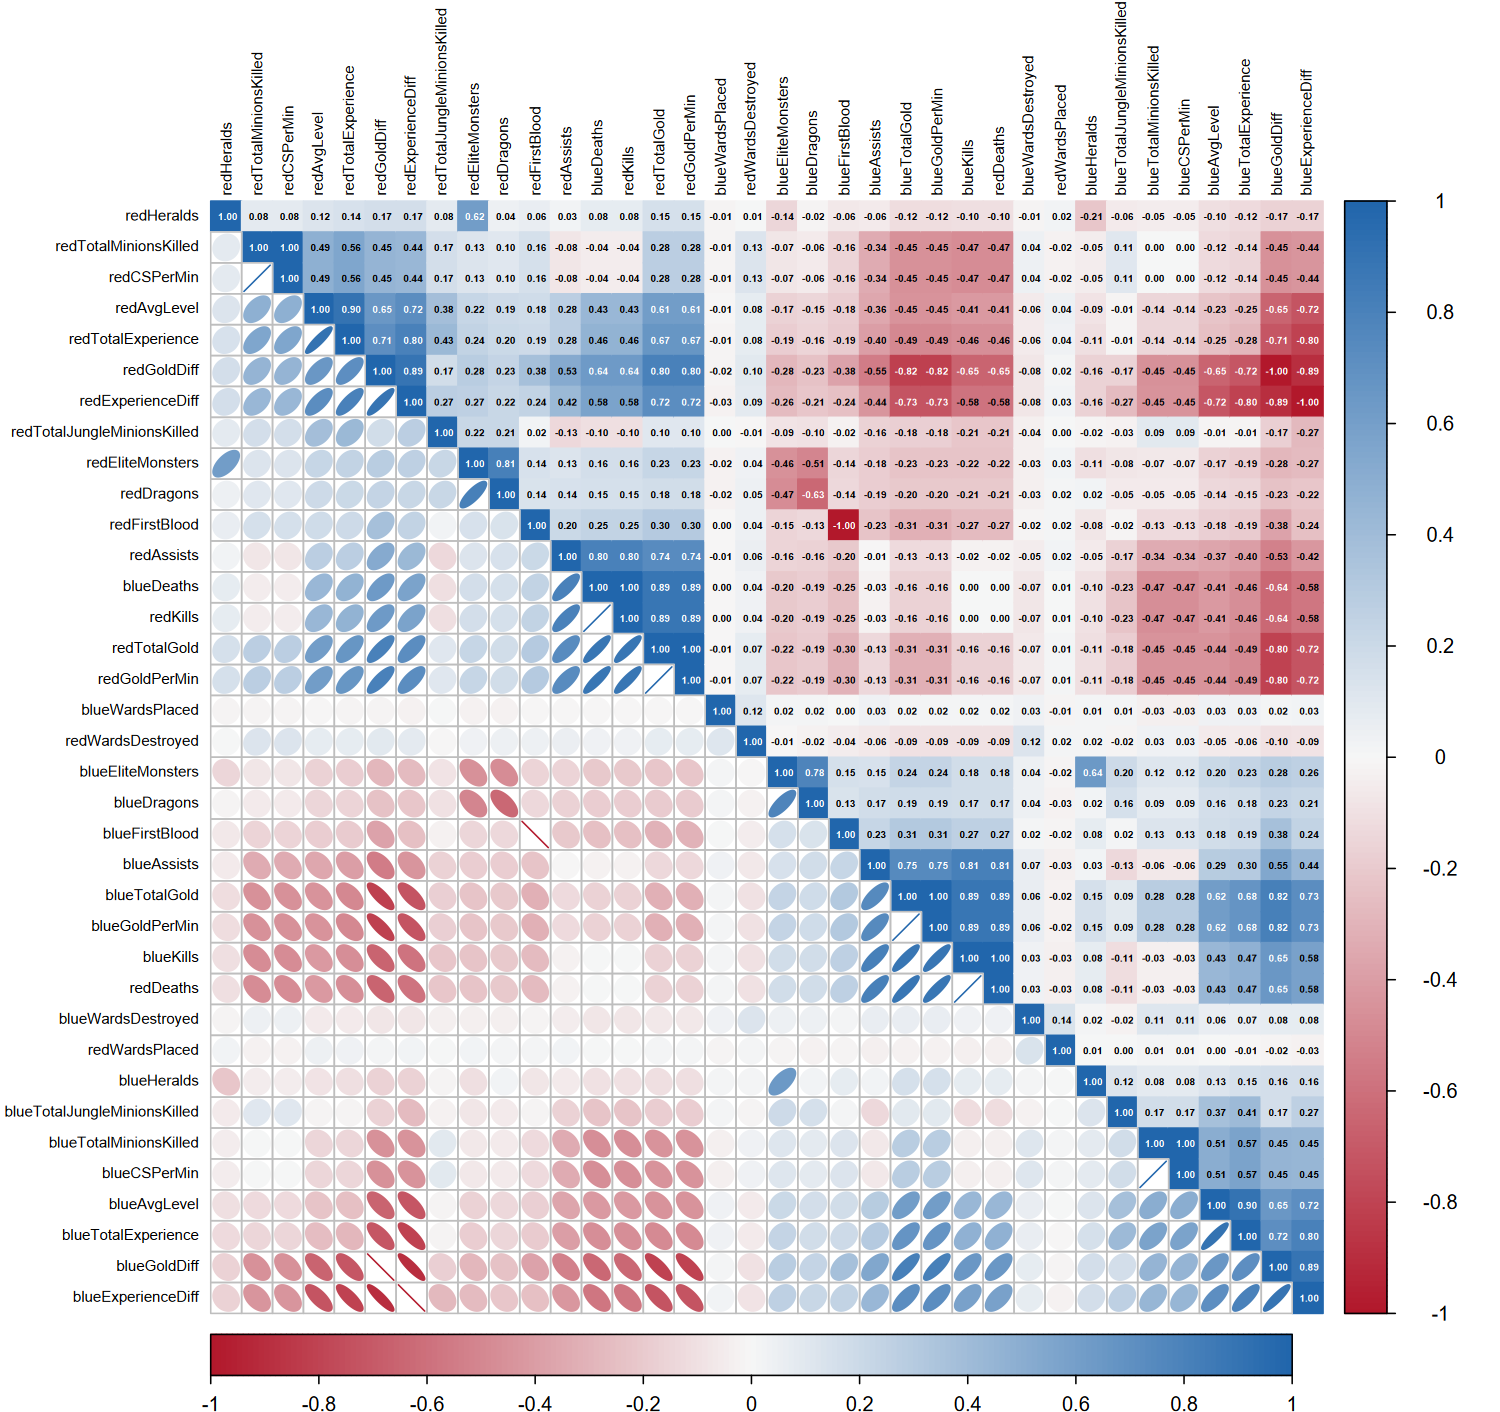
\includegraphics[width=1.0\textwidth]{../Plots/corrmatrixes/WykresKorelacji1.png}
	}
	\caption{Macierz korelacji dla wszystkich zmiennych bez quasi stałych 1.}
\end{figure}
\begin{samepage}
\indent Powyższa macierz przedstawia korelacje liniowe, proste pomiędzy wszystkimi zmiennymi, jakie nam zostały po usunięciu quasi stałych. Na jego postawie możemy znaleźć bardzo silnie skorelowane, czyli takie, których poziom korelacji jest większy bądź równy 0.9, pary cech:
\begin{table}[H]
  \centering
\begin{tabular}{l l c}
	\toprule
	\textbf{Cecha A} & \textbf{Cecha B} &  \textbf{Korelacja A i B}  \\
	\midrule
	blueFirstBlood & redFirstBlood & -1 \\ 
	redDeaths  &  blueKills & 1 \\
	blueDeaths  & redKills  & 1 \\
	blueTotalGold  & blueGoldPerMin &  1 \\
	blueAvgLevel  & blueTotalExperience &  0.901297 \\
	blueTotalMinionsKilled  & blueCSPerMin  & 1 \\
	blueGoldDiff &  redGoldDiff  & -1 \\
	blueExperienceDiff  & redExperienceDiff  & -1 \\
	redTotalGold &  redGoldPerMin &  1 \\
	redAvgLevel  & redTotalExperience &  0.901748 \\
	redTotalMinionsKilled &  redCSPerMin  & 1 \\
	\bottomrule
\end{tabular}
\caption{Tabela korelacji silnie skorelowanych zmiennych 1.}
\end{table}
\end{samepage}
\begin{samepage}
\indent Na podstawie powyższego możemy usunąć następujące cech;
\begin{itemize}
	\item blueFirstBlood
	\item redDeaths
	\item blueDeaths  
	\item blueTotalGold  
	\item blueAvgLevel  
	\item blueTotalMinionsKilled  
	\item blueGoldDiff 
	\item blueExperienceDiff  
	\item redTotalGold 
	\item redAvgLevel 
	\item redTotalMinionsKilled 
\end{itemize}
\end{samepage}
\begin{samepage}
\subsubsection{Skorelowane wielokrotnie, liniowo}
\indent \indent Dodatkowo, możemy, korzystając z definicji poszczególnych cech, zebrać korelacje wielokrotne, liniowe; innymi słowy takie korelacje, w których to jedna zmienna jest skorelowana liniowo z więcej niż jedną. Takich relacji mamy aż 6 i są one przedstawione poniżej:
\begin{itemize}
	\item $blueEliteMonsters = blueDragons + blueHeralds$
	\item $redEliteMonsters = redDragons + redHeralds$
	\item $blueGoldDiff = blueTotalGold - redTotalGold$ gdzie blueGoldDiff został już usunięty
	\item $redGoldDiff = redTotalGold - blueTotalGold$
	\item $blueExperienceDiff = blueTotalExperience - redTotalExperience$ gdzie blueExperienceDiff został już usunięty
	\item $redExperienceDiff = redTotalExperience - blueTotalExperience$
\end{itemize}
\end{samepage}
\begin{samepage}
\indent \indent Na podstawie wyżej wymienionych relacji usuwamy następujące zmienne:
\begin{itemize}
	\item $blueEliteMonsters$ i $redEliteMonsters$ jako że istnieje potencjalnie istotna różnica pomiędzy zabiciem heralda a smoka i dlatego wolimy zostawić zmienne z wymienionymi skorelowane
	\item $blueGoldPerMin$ i $redGoldPerMin$ jako że są one liniowo skorelowane odpowiednio z $blueTotalGold$ i $redTotalGold$ oraz przez wzgląd na to, że uznajemy różnicę między nimi za istotniejszą od tych zmiennych samych w sobie
	\item $blueTotalExperience$ i $redTotalExperience$ jako że uznajemy różnicę między nimi za istotniejszą od tych zmiennych samych w sobie
\end{itemize}
\end{samepage}

\subsection{Łączenie zmiennych}
\indent \indent Po porzedniej podsekcji zostały nam cechy przedstawione na narysowanej poniżej macierzy korelacji:
\begin{figure}[H]
	\centering
	\makebox[\textwidth][c]{%
		\includegraphics[width=1.0\textwidth]{../Plots/corrmatrixes/WykresBezElite.png}
	}
	\caption{Macierz korelacji dla wszystkich zmiennych po usuwaniu liniowo skorelowanych}
\end{figure}
\pagebreak

\begin{samepage}
\subsubsection{Agregacja}
\indent \indent Jak można wyczytać z powyższej macierzy, mamy 3 pary silnie skorelowanych cech. Spośród nich 2 to następujące pary:
\begin{table}[H]
  \centering
\begin{tabular}{l l c}
	\toprule
	\textbf{Cecha A} & \textbf{Cecha B} &  \textbf{Korelacja A i B}  \\
	\midrule
	redKills & redAssists & 0.8 \\ 
	blueKills  &  blueAssists & 0.81 \\
	\bottomrule
\end{tabular}
\caption{Tabela korelacji silnie skorelowanych zmiennych 2.}
\end{table}
\indent Te cechy zagragujemy liniowo w jedną, dla każdej drużyny, wedle następującej reguły:
\begin{equation}
	KA = Kills + Assists
\end{equation}

\indent Tym samym otrzymujemy następujące nowe cechy:
\begin{itemize}
	\item blueKA
	\item redKA
\end{itemize}
\end{samepage}
\begin{samepage}
\subsubsection{PCA}
\indent \indent Po agregacji została nam następująca para cech silnie skorelowanych:
\begin{table}[H]
  \centering
\begin{tabular}{l l c}
	\toprule
	\textbf{Cecha A} & \textbf{Cecha B} &  \textbf{Korelacja A i B}  \\
	\midrule
	redGoldDiff & redExperienceDiff & 0.89 \\ 
	\bottomrule
\end{tabular}
\caption{Tabela korelacji silnie skorelowanych zmiennych 3.}
\end{table}
\indent \indent Do zagregowania tych zmiennych wykorzystamy metodę PCA. Poniżej przedstawimy, opis tej metody:
\newline 

Niech macierz danych będzie opisana jako:
\begin{equation}
\mathbf{X} \in \mathbb{R}^{n \times p},
\end{equation}
gdzie $n$ oznacza liczbę obserwacji, a $p$ liczbę zmiennych. Metoda PCA przekształca pierwotny zbiór $p$ skorelowanych zmiennych w nowy zbiór zmiennych, zwanych \textbf{głównymi składowymi}, które są wzajemnie nieskorelowane i uporządkowane według malejącej wariancji.

W pierwszym kroku dane są zwykle centrowane, a w przypadku zmiennych mierzonych w różnych skalach również standaryzowane. Następnie wyznacza się macierz kowariancji:
\begin{equation}
\mathbf{S} = \frac{1}{n-1}\mathbf{X}^\top \mathbf{X},
\end{equation}
lub, w przypadku danych standaryzowanych, macierz korelacji.

Kolejnym etapem jest wyznaczenie wartości własnych i wektorów własnych macierzy $\mathbf{S}$:
\begin{equation}
\mathbf{S}\mathbf{v}_k = \lambda_k \mathbf{v}_k,
\end{equation}
gdzie $\lambda_k$ oznacza $k$-tą wartość własną, a $\mathbf{v}_k$ odpowiadający jej wektor własny. Wektory własne wyznaczają kierunki głównych składowych, natomiast wartości własne informują o ilości wariancji wyjaśnianej przez każdą składową.

Główne składowe wyznacza się jako liniowe kombinacje zmiennych pierwotnych:
\begin{equation}
\mathbf{z}_k = \mathbf{X}\mathbf{v}_k.
\end{equation}
Pierwsza główna składowa wyjaśnia największą możliwą część wariancji danych, druga -- największą część pozostałej wariancji, przy zachowaniu ortogonalności względem pierwszej, itd.

Redukcja wymiarowości polega na wyborze pierwszych $m$ składowych, gdzie $m < p$, tak aby zachować jak największą część całkowitej zmienności danych. Udział wariancji wyjaśnionej przez $k$-tą składową można obliczyć jako:
\begin{equation}
\frac{\lambda_k}{\sum_{j=1}^{p}\lambda_j}.
\end{equation}
Z kolei skumulowany udział wyjaśnionej wariancji dla pierwszych $m$ składowych wynosi:
\begin{equation}
\frac{\sum_{k=1}^{m}\lambda_k}{\sum_{j=1}^{p}\lambda_j}.
\end{equation}

W praktyce wybiera się taką liczbę składowych, aby skumulowana wariancja osiągała założony poziom, np. $80\%$, $90\%$ lub $95\%$. Dzięki temu możliwe jest zastąpienie dużej liczby zmiennych mniejszym zbiorem nowych cech, co upraszcza analizę, zmniejsza złożoność modeli oraz ogranicza problem współliniowości.

W skrypcie będziemy bazować na wbudowanej funkcji "prcomp" i do wizualizacji rzutu wykorzystamy funkcję "fviz\_pca\_biplot" z biblioteki factoextra. Poniżej przedstawiony jest wykres po zastosowaniu PCA.
\end{samepage}
\begin{figure}[H]
	\centering
	\makebox[\textwidth][c]{%
		\includegraphics[width=1\textwidth]{../Plots/PCA/biplot_diff.png}
	}
	\caption{Wykres PCA dla cech redGoldDiff i redExperienceDiff}
\end{figure}
\indent \indent Jak na załączonym wyżej obrazku widać, nowa cecha, roboczo nazwana $Dim1$, odpowiada za aż około 94.7\% wariancji. Stąd też możemy uznać, że taka agregacja będzie dobrą formą wyeliminowania silnej korelacji. Od tego momentu zmienna robocza nazwana $Dim1$ będzie miała nazwę $dif$\_$PCA$\_$Component$\_$1$.

\indent Po wykonaniu wszystkich kroków usuwania silnie i bardzo silnie skorelowanych cech możemy przedstawić jak ostatecznie wygląda macierz korelacji. Dodatkowo macierz uwzględnia cechę $blueWins$, aby dodatkowo ukazać jak silnie jest ona skorelowana ze zmiennymi, które ostatecznie zostały.

\section{Analiza końcowego zbioru danych}
\subsection{Wyjaśnienie zmiennych}
\begin{itemize}
	\item {\bf blueWardsPlaced} --- Ilość wardów postawionych przez druyżynę niebieską.
	\item {\bf blueWardsDestroyed} --- Ilość wardów zniszczonych przez druyżynę niebieską. 
	\item {\bf blueDragons} --- Liczba smoków zabitych przez drużynę niebieską.
	\item {\bf blueHeralds} --- Liczba Heroldów zabitych przez drużynę niebieską.
	\item {\bf blueTotalJungleMinionsKilled} --- Łączna ilość zabitych minionów z dżungli przez drużynę niebieską.
	\item {\bf blueCSPerMin} --- Ilość zabitych minionów przez drużnę niebieską w przeliczeniu na minute.
	\item {\bf redWardsPlaced} --- Ilość wardów postawionych przez druyżynę czerwoną.
	\item {\bf redWardsDestroyed} ---  Ilość wardów zniszczonych przez druyżynę czerwoną. 
	\item {\bf redFirstBlood} --- Informacja o zdobyciu pierwszego zabójstwa (First Blood) przez drużynę czerwoną.
	\item {\bf redDragons} ---  Liczba smoków zabitych przez drużynę czerwoną.
	\item {\bf redHeralds} --- Liczba Heroldów zabitych przez drużynę czerwoną.
	\item {\bf redTotalJungleMinionsKilled} --- Łączna ilość zabitych minionów z dżungli przez drużynę czerwoną.
	\item {\bf redCSPerMin} --- Ilość zabitych minionów przez drużnę czerwoną w przeliczeniu na minute.
	\item {\bf blueKA} --- Łączna ilość zabójstw i asyst drużyny niebieskiej.
	\item {\bf redKA} --- Łączna ilość zabójstw i asyst drużyny czerwonej.
	\item {\bf diff\_PCA\_Component\_1} --- Nowa zmienna utworzona w procesie PCA ze zmiennych \textit{redGoldDiff} i \textit{redExperienceDiff}.
\end{itemize}

\subsection{Charakterystyka zmiennych}
Zmienne opisujące opisujące ilość zabitych smoków i heroldów powinny być zmiennymi numerycznymi jednak przez ograniczoną naturę badanego zbioru danych przyjmują jedynie wartości 0 lub 1. Z tego powodu zostały one opisane jako zmienne binarne.
\begin{table}[H]
\centering
\begin{tabular}{l l l l}
\toprule
	\textbf{Zmienna} & \textbf{Typ} & \textbf{Skala} & \textbf{Charakter} \\
\midrule
	blueWardsPlaced & Numeryczna & Ilościowa & Skokowa \\
	blueWardsDestroyed & Numeryczna & Ilościowa & Skokowa \\
	blueDragons & Binarna & Nominalna & Skokowa \\
	blueHeralds & Binarna & Nominalna & Skokowa \\
	blueTotalJungleMinionsKilled & Numeryczna & Ilościowa & Skokowa \\
	blueCSPerMin & Numeryczna & Ilościowa & Ciągła \\
	redWardsPlaced & Numeryczna & Ilościowa & Skokowa \\
	redWardsDestroyed & Numeryczna & Ilościowa & Skokowa \\
	redFirstBlood & Binarna & Nominalna & Skokowa \\
	redDragons & Binarna & Nominalna & Skokowa \\
	redHeralds & Binarna & Nominalna & Skokowa \\
	redTotalJungleMinionsKilled & Numeryczna & Ilościowa & Skokowa \\
	redCSPerMin & Numeryczna & Ilościowa & Ciągła \\
	blueKA & Numeryczna & Ilościowa & Skokowa \\
	redKA & Numeryczna & Ilościowa & Skokowa \\
	diff\_PCA\_Component\_1 & Numeryczna & Ilościowa & Ciągła \\
\bottomrule
\end{tabular}
\caption{Charakterystyka końcowych zmiennych.}
\end{table}

\subsection{Statystyki opisowe}
\begin{table}[H]
\centering
\resizebox{\textwidth}{!}{
\begin{tabular}{l c c c c c c c c c c c}
\toprule
	\textbf{Zmienna} & \textbf{Średnia} & \textbf{Mediana} & \textbf{Min.} & \textbf{Maks.} & \textbf{Odch. std.}  & \textbf{Skośność} \\
\midrule
	blueWardsPlaced & 0.00 & -0.37 & -1.16 & 6.02 & 1.00 & 2.94 \\
	blueWardsDestroyed & 0.00 & 0.08 & -1.30 & 11.10 & 1.00 & 2.85 \\
	blueDragons & 0.36 & 0.00 & 0.00 & 1.00 & 0.48 & 0.57 \\
	blueHeralds & 0.19 & 0.00 & 0.00 & 1.00 & 0.39 & 1.60 \\
	blueTotalJungleMinionsKilled & 0.00 & -0.05 & -5.09 & 4.19 & 1.00 & 0.12 \\
	blueCSPerMin & 0.00 & 0.06 & -5.79 & 3.03 & 1.00 & -0.26 \\
	redWardsPlaced & 0.00 & -0.38 & -1.12 & 6.11 & 1.00 & 2.81 \\
	redWardsDestroyed & 0.00 & -0.34 & -1.27 & 9.92 & 1.00 & 2.95 \\
	redFirstBlood & 0.50 & 0.00 & 0.00 & 1.00 & 0.50 & 0.02 \\
	redDragons & 0.41 & 0.00 & 0.00 & 1.00 & 0.49 & 0.35 \\
	redHeralds & 0.16 & 0.00 & 0.00 & 1.00 & 0.37 & 1.86 \\
	redTotalJungleMinionsKilled & 0.00 & -0.03 & -4.71 & 4.05 & 1.00 & 0.23 \\
	redCSPerMin & 0.00 & 0.03 & -5.04 & 3.26 & 1.00 & -0.29 \\
	blueKA & 0.00 & -0.12 & -1.90 & 5.66 & 1.00 & 0.69 \\
	redKA & 0.00 & -0.12 & -1.92 & 4.54 & 1.00 & 0.63 \\
	diff\_PCA\_Component\_1 & 0.00 & 0.00 & -4.61 & 4.75 & 1.00 & -0.03 \\
\bottomrule
\end{tabular}
}
\caption{Statystyki opisowe końcowych zmiennych.}
\end{table}

\subsection{Wizualizacja}
Poniżej przedstawiono wizualizacje zmiennych po wstępnej analizie danych z pominięciem skalowania dla zachowania czytelności wykresów.
%%%%%%%%%%%%%%%%%%%%%%%%%%%%%%%%%%%%%%%%%%%%%%%%%%%%%%%%%%%%%%%%%
\begin{figure}[H]
	\centering
	\makebox[\textwidth][c]{%
		\includegraphics[width=1.0\textwidth]{../Plots/corrmatrixes/WykresZblueWins.png}
	}
	\caption{Macierz korelacji dla ostatecznych zmiennych oraz dla zmiennej przewidywanej \textit{blueWins}.}
\end{figure}

    \begin{figure}[H]
        \centering
        \includegraphics[height=0.33\textwidth]{../Plots/boxplots/box_blueWardsPlaced.png}
        \hfill
        \includegraphics[height=0.33\textwidth]{../Plots/histograms_and_barplots/hist_blueWardsPlaced.png}
        \caption{Boxplot oraz histogram z nałożoną funkcją gęstości dla zmiennej blueWardsPlaced.}
        \label{fig:both_images}
    \end{figure}
    

    \begin{figure}[H]
        \centering
        \includegraphics[height=0.33\textwidth]{../Plots/boxplots/box_blueWardsDestroyed.png}
        \hfill
        \includegraphics[height=0.33\textwidth]{../Plots/histograms_and_barplots/bar_blueWardsDestroyed.png}
        \caption{Boxplot oraz barplot dla zmiennej blueWardsDestroyed.}
        \label{fig:both_images}
    \end{figure}
    

    \begin{figure}[H]
        \centering
        \includegraphics[height=0.33\textwidth]{../Plots/boxplots/box_blueTotalJungleMinionsKilled.png}
        \hfill
        \includegraphics[height=0.33\textwidth]{../Plots/histograms_and_barplots/hist_blueTotalJungleMinionsKilled.png}
        \caption{Boxplot oraz histogram z nałożoną funkcją gęstości dla zmiennej blueTotalJungleMinionsKilled.}
        \label{fig:both_images}
    \end{figure}
    

    \begin{figure}[H]
        \centering
        \includegraphics[height=0.33\textwidth]{../Plots/boxplots/box_blueCSPerMin.png}
        \hfill
        \includegraphics[height=0.33\textwidth]{../Plots/histograms_and_barplots/hist_blueCSPerMin.png}
        \caption{Boxplot oraz histogram z nałożoną funkcją gęstości dla zmiennej blueCSPerMin.}
        \label{fig:both_images}
    \end{figure}
    

    \begin{figure}[H]
        \centering
        \includegraphics[height=0.33\textwidth]{../Plots/boxplots/box_redWardsPlaced.png}
        \hfill
        \includegraphics[height=0.33\textwidth]{../Plots/histograms_and_barplots/hist_redWardsPlaced.png}
        \caption{Boxplot oraz histogram z nałożoną funkcją gęstości dla zmiennej redWardsPlaced.}
        \label{fig:both_images}
    \end{figure}
    

    \begin{figure}[H]
        \centering
        \includegraphics[height=0.33\textwidth]{../Plots/boxplots/box_redWardsDestroyed.png}
        \hfill
        \includegraphics[height=0.33\textwidth]{../Plots/histograms_and_barplots/bar_redWardsDestroyed.png}
        \caption{Boxplot oraz barplot dla zmiennej redWardsDestroyed.}
        \label{fig:both_images}
    \end{figure}
    

    \begin{figure}[H]
        \centering
        \includegraphics[height=0.33\textwidth]{../Plots/boxplots/box_redTotalJungleMinionsKilled.png}
        \hfill
        \includegraphics[height=0.33\textwidth]{../Plots/histograms_and_barplots/hist_redTotalJungleMinionsKilled.png}
        \caption{Boxplot oraz histogram z nałożoną funkcją gęstości dla zmiennej redTotalJungleMinionsKilled.}
        \label{fig:both_images}
    \end{figure}
    

    \begin{figure}[H]
        \centering
        \includegraphics[height=0.33\textwidth]{../Plots/boxplots/box_redCSPerMin.png}
        \hfill
        \includegraphics[height=0.33\textwidth]{../Plots/histograms_and_barplots/hist_redCSPerMin.png}
        \caption{Boxplot oraz histogram z nałożoną funkcją gęstości dla zmiennej redCSPerMin.}
        \label{fig:both_images}
    \end{figure}
    

    \begin{figure}[H]
        \centering
        \includegraphics[height=0.33\textwidth]{../Plots/boxplots/box_blueKA.png}
        \hfill
        \includegraphics[height=0.33\textwidth]{../Plots/histograms_and_barplots/bar_blueKA.png}
        \caption{Boxplot oraz barplot dla zmiennej blueKA.}
        \label{fig:both_images}
    \end{figure}
    

    \begin{figure}[H]
        \centering
        \includegraphics[height=0.33\textwidth]{../Plots/boxplots/box_redKA.png}
        \hfill
        \includegraphics[height=0.33\textwidth]{../Plots/histograms_and_barplots/bar_redKA.png}
        \caption{Boxplot oraz barplot dla zmiennej redKA.}
        \label{fig:both_images}
    \end{figure}
    

    \begin{figure}[H]
        \centering
        \includegraphics[height=0.33\textwidth]{../Plots/boxplots/box_diff_PCA_Component_1.png}
        \hfill
        \includegraphics[height=0.33\textwidth]{../Plots/histograms_and_barplots/hist_diff_PCA_Component_1.png}
        \caption{Boxplot oraz histogram z nałożoną funkcją gęstości dla zmiennej diff\_PCA\_Component\_1.}
        \label{fig:both_images}
    \end{figure}

%%%%%%%%%%%%%%%%%%%%%%%%%%%%%%%%%%%%%%%%%%%%%%%%%%%%%%%%%%%%%%%%%

    \begin{figure}[H]
        \centering
        \includegraphics[height=0.33\textwidth]{../Plots/piecharts/pie_blueDragons.png}
        \hfill
        \includegraphics[height=0.33\textwidth]{../Plots/piecharts/pie_redDragons.png}
	\caption{Piecharty dla zmiennych blueDragons oraz redDragons.}
        \label{fig:both_images}
    \end{figure}

    \begin{figure}[H]
        \centering
        \includegraphics[height=0.33\textwidth]{../Plots/piecharts/pie_blueHeralds.png}
        \hfill
        \includegraphics[height=0.33\textwidth]{../Plots/piecharts/pie_redHeralds.png}
	\caption{Piecharty dla zmiennych blueHeralds oraz redHeralds.}
        \label{fig:both_images}
    \end{figure}

    \begin{figure}[H]
        \centering
        \includegraphics[height=0.33\textwidth]{../Plots/piecharts/pie_redFirstBlood.png}
	\caption{Piechart dla zmiennej redFirstBlood.}
        \label{fig:both_images}
    \end{figure}

%%%%%%%%%%%%%%%%%%%%%%%%%%%%%%%%%%%%%%%%%%%%%%%%%%%%%%%%%%%%%%%%%

\section{Opisy metod}
%%%%%%%%%%%%%%%%%%%%%%%%%%%%%%%%%%%%%%%%%%%%%%%%%%%%%%%%%%%%%%%%%
\subsection{Sieci neuronowe}

\subsubsection{Opis}

Sieci neuronowe są modelami uczenia maszynowego inspirowanymi działaniem biologicznych sieci neuronowych. Składają się z połączonych ze sobą neuronów tworzących kolejne warstwy przetwarzające dane wejściowe. Dzięki zastosowaniu nieliniowych funkcji aktywacji sieci neuronowe są zdolne do modelowania złożonych zależności pomiędzy zmiennymi.

W analizie wykorzystano wielowarstwową sieć neuronową typu MLP (Multi-Layer Perceptron) zaimplementowaną przy użyciu bibliotek \texttt{keras3} oraz \texttt{tensorflow}. Zadaniem modelu było przewidywanie wartości zmiennej \texttt{blueWins}, określającej końcowy wynik meczu z perspektywy drużyny niebieskiej.

Dla wektora wejściowego $\mathbf{x}$ predykcja modelu może zostać zapisana jako:

\begin{equation}
\hat{y} = \sigma(f(\mathbf{x}, \theta))
\end{equation}

gdzie:
\begin{itemize}
\item $\mathbf{x}$ -- wektor cech wejściowych,
\item $\theta$ -- zbiór parametrów modelu,
\item $f(\cdot)$ -- transformacja realizowana przez warstwy ukryte,
\item $\sigma(\cdot)$ -- funkcja sigmoidalna.
\end{itemize}

Funkcja sigmoidalna przyjmuje postać:

\begin{equation}
\sigma(z)=\frac{1}{1+e^{-z}}
\end{equation}

i zwraca wartość z przedziału $[0,1]$, interpretowaną jako prawdopodobieństwo przynależności do klasy pozytywnej.

Zastosowana architektura składała się z czterech warstw:
\begin{itemize}
\item warstwy wejściowej zawierającej 16 cech,
\item pierwszej warstwy ukrytej zawierającej 128 neuronów z funkcją aktywacji ELU,
\item drugiej warstwy ukrytej zawierającej 64 neurony z funkcją aktywacji Softplus,
\item warstwy wyjściowej zawierającej jeden neuron z funkcją sigmoidalną.
\end{itemize}

W celu ograniczenia zjawiska przeuczenia pomiędzy warstwami zastosowano mechanizm \textit{dropout} z parametrem $p=0.5$, polegający na losowym wyłączaniu części neuronów podczas procesu uczenia.

\subsubsection{Funkcja straty}

Proces uczenia polegał na minimalizacji funkcji straty binary cross-entropy:

\begin{equation}
L = -\frac{1}{N}\sum_{i=1}^{N}
\left[
y_i \log(\hat{y}_i)
+
(1-y_i)\log(1-\hat{y}_i)
\right]
\end{equation}

gdzie:
\begin{itemize}
\item $N$ -- liczba obserwacji,
\item $y_i$ -- rzeczywista wartość klasy,
\item $\hat{y}_i$ -- prawdopodobieństwo przewidziane przez model.
\end{itemize}

Minimalizacja funkcji straty była realizowana przy użyciu algorytmu RMSprop, który adaptacyjnie dostosowuje współczynnik uczenia na podstawie historii gradientów.

\subsubsection{Proces uczenia}

Dane zostały losowo podzielone na zbiór treningowy (70\% obserwacji) oraz testowy (30\% obserwacji). Model trenowano przez 50 epok przy wielkości batcha wynoszącej 100 obserwacji.

Po zakończeniu procesu uczenia wyznaczono prawdopodobieństwa przynależności do klasy pozytywnej dla obserwacji ze zbioru testowego. Otrzymane wartości zostały następnie wykorzystane do oceny jakości klasyfikacji przy użyciu miar opisanych w sekcji dotyczącej metod oceniania.


%%%%%%%%%%%%%%%%%%%%%%%%%%%%%%%%%%%%%%%%%%%%%%%%%%%%%%%%%%%%%%%%%
\subsection{Drzewo klasyfikacyjne}

\subsubsection{Opis}

Drzewo decyzyjne [?] jest metodą klasyfikacji wykorzystującą strukturę hierarchiczną składającą się z węzłów decyzyjnych oraz liści reprezentujących klasy. Celem algorytmu jest podział przestrzeni cech na obszary możliwie jednorodne pod względem zmiennej decyzyjnej.

Proces budowy drzewa rozpoczyna się od umieszczenia wszystkich obserwacji w węźle korzeniowym. Następnie wykonywane są kolejne podziały zbioru danych na podstawie wartości wybranych cech. W każdym kroku wybierany jest taki podział, który prowadzi do największego zwiększenia jednorodności klas w otrzymanych podzbiorach.

Algorytm budowy drzewa można przedstawić w postaci następujących kroków:

\begin{enumerate}
    \item Umieszczenie wszystkich obserwacji w węźle korzeniowym.
    \item Wyznaczenie najlepszego podziału dla każdej dostępnej cechy.
    \item Wybór podziału maksymalizującego jakość rozdzielenia klas.
    \item Utworzenie nowych węzłów potomnych.
    \item Powtarzanie kroków 2--4 aż do spełnienia kryterium zatrzymania.
\end{enumerate}

W analizie wykorzystano drzewo klasyfikacyjne służące do przewidywania wartości zmiennej \texttt{blueWins}, określającej końcowy wynik meczu z perspektywy drużyny niebieskiej.

Dane zostały losowo podzielone na zbiór treningowy (70\% obserwacji) oraz testowy (30\% obserwacji). Model został wytrenowany na zbiorze treningowym, natomiast jego skuteczność oceniono na niezależnym zbiorze testowym. Dodatkowo podczas procesu przycinania drzewa wykorzystano walidację krzyżową w celu wyznaczenia optymalnego rozmiaru modelu i ograniczenia zjawiska przeuczenia.


\subsubsection{Kryterium podziału}

Podczas budowy drzewa zastosowano kryterium dewiancji, wykorzystywane przez bibliotekę \texttt{tree}. Dla pojedynczego węzła dewiancja definiowana jest jako:

\begin{equation}
D = -2 \sum_{i=1}^{K} n_i \ln(p_i)
\end{equation}

gdzie:
\begin{itemize}
    \item $K$ -- liczba klas,
    \item $n_i$ -- liczba obserwacji należących do klasy $i$,
    \item $p_i$ -- prawdopodobieństwo wystąpienia klasy $i$ w analizowanym węźle.
\end{itemize}

Optymalny podział jest wybierany w taki sposób, aby maksymalnie zmniejszyć całkowitą dewiancję drzewa.

\subsubsection{Przycinanie drzewa}

Drzewa decyzyjne są podatne na przeuczenie (\textit{overfitting}), szczególnie gdy ich struktura staje się zbyt rozbudowana. W celu ograniczenia tego zjawiska zastosowano proces przycinania drzewa (\textit{pruning}).

Przycinanie polega na usuwaniu części gałęzi, które nie wnoszą istotnej informacji predykcyjnej. W pracy optymalny rozmiar drzewa został wyznaczony z wykorzystaniem walidacji krzyżowej. Spośród analizowanych struktur wybierano model minimalizujący błąd klasyfikacji na danych walidacyjnych.

%%%%%%%%%%%%%%%%%%%%%%%%%%%%%%%%%%%%%%%%%%%%%%%%%%%%%%%%%%%%%%%%%
\subsection{K najbliższych sąsiadów}

\subsubsection{Opis}

Metoda k najbliższych sąsiadów (ang. \textit{k-Nearest Neighbours}, KNN) należy do grupy metod klasyfikacji opartych na podobieństwie obserwacji. Klasyfikacja nowego obiektu odbywa się na podstawie klas przypisanych do $k$ najbardziej podobnych obserwacji ze zbioru treningowego.

Dla każdej obserwacji testowej wyznaczani są jej najbliżsi sąsiedzi w przestrzeni cech, a następnie przypisywana jest klasa najczęściej występująca wśród znalezionych sąsiadów. Metoda nie tworzy jawnego modelu podczas etapu uczenia, dlatego zaliczana jest do grupy metod leniwych (ang. \textit{lazy learning}).

W analizie wykorzystano algorytm KNN zaimplementowany w bibliotekach \texttt{caret} oraz \texttt{class}. Dane zostały losowo podzielone na zbiór treningowy (70\% obserwacji) oraz testowy (30\% obserwacji). Model został zbudowany na zbiorze treningowym, natomiast jego skuteczność oceniono na niezależnym zbiorze testowym.

\subsubsection{Miara odległości}

Kluczowym elementem algorytmu KNN jest wyznaczenie odległości pomiędzy obserwacjami. W analizie wykorzystano odległość euklidesową:

\begin{equation}
d(\mathbf{x}, \mathbf{y}) =
\sqrt{
\sum_{j=1}^{p}
(x_j-y_j)^2
}
\end{equation}

gdzie:
\begin{itemize}
    \item $\mathbf{x}$ oraz $\mathbf{y}$ -- porównywane obserwacje,
    \item $p$ -- liczba cech,
    \item $x_j$, $y_j$ -- wartości $j$-tej cechy.
\end{itemize}

Na podstawie obliczonych odległości wybieranych jest $k$ najbliższych sąsiadów analizowanej obserwacji.

\subsubsection{Dobór parametru \texorpdfstring{$k$}{k}}

Jednym z najważniejszych parametrów algorytmu jest liczba sąsiadów $k$. Zbyt małe wartości mogą prowadzić do nadmiernego dopasowania modelu do danych treningowych, natomiast zbyt duże mogą powodować utratę zdolności rozróżniania klas.

W celu wyznaczenia optymalnej wartości parametru $k$ zastosowano dziesięciokrotną walidację krzyżową. Analizowano wyłącznie nieparzyste wartości parametru z przedziału od 1 do 101:

\[
k \in \{1,3,5,\ldots,101\}
\]

Jako wartość końcową przyjęto parametr zapewniający najwyższą skuteczność klasyfikacji podczas walidacji krzyżowej.

\subsubsection{Reguła klasyfikacji}

Klasa nowej obserwacji wyznaczana jest na podstawie głosowania większościowego wśród $k$ najbliższych sąsiadów:

\begin{equation}
\hat{y} =
\arg\max_{c \in C}
\sum_{i \in N_k}
I(y_i = c)
\end{equation}

gdzie:
\begin{itemize}
    \item $C$ -- zbiór możliwych klas,
    \item $N_k$ -- zbiór $k$ najbliższych sąsiadów,
    \item $I(\cdot)$ -- funkcja wskaźnikowa przyjmująca wartość 1, gdy warunek jest spełniony, oraz 0 w przeciwnym przypadku.
\end{itemize}

Oprócz przewidywanej klasy algorytm wyznacza również prawdopodobieństwo przynależności do klasy pozytywnej, obliczane jako udział sąsiadów należących do tej klasy.

%%%%%%%%%%%%%%%%%%%%%%%%%%%%%%%%%%%%%%%%%%%%%%%%%%%%%%%%%%%%%%%%%
\subsection{Opis metody hybrydowej}
%%%%%%%%%%%%%%%%%%%%%%%%%%%%%%%%%%%%%%%%%%%%%%%%%%%%%%%%%%%%%%%%%
\subsection{Metody oceniania}

Ocena jakości modeli klasyfikacyjnych stanowi istotny element analizy, ponieważ pozwala na porównanie skuteczności zastosowanych metod oraz określenie ich przydatności w kontekście rozważanego problemu predykcji wyniku meczu. W niniejszej pracy wykorzystano miary oparte na macierzy pomyłek oraz krzywą ROC wraz z polem pod krzywą AUC.

\subsubsection{Macierz pomyłek i miary klasyfikacji}

Podstawą oceny modeli klasyfikacyjnych jest macierz pomyłek, która zestawia rzeczywiste klasy obserwacji z klasami przewidzianymi przez model. Dla problemu binarnej klasyfikacji wyróżnia się cztery podstawowe wartości:

\begin{itemize}
    \item $TP$ (True Positive) -- liczba poprawnie przewidzianych przypadków pozytywnej klasy,
    \item $TN$ (True Negative) -- liczba poprawnie przewidzianych przypadków negatywnej klasy,
    \item $FP$ (False Positive) -- liczba błędnie przewidzianych przypadków pozytywnej klasy,
    \item $FN$ (False Negative) -- liczba błędnie przewidzianych przypadków negatywnej klasy.
\end{itemize}

Na podstawie macierzy pomyłek definiuje się następujące miary jakości klasyfikacji:

\textbf{Dokładność (Accuracy)} określająca odsetek poprawnych klasyfikacji:

\begin{equation}
Accuracy = \frac{TP + TN}{TP + TN + FP + FN}
\end{equation}

\textbf{Precyzja (Precision)} określająca, jak wiele przewidzianych przypadków pozytywnych jest rzeczywiście poprawnych:

\begin{equation}
Precision = \frac{TP}{TP + FP}
\end{equation}

\textbf{Czułość (Sensitivity, Recall)} określająca zdolność modelu do wykrywania pozytywnych przypadków:

\begin{equation}
Sensitivity = \frac{TP}{TP + FN}
\end{equation}

\textbf{Specyficzność (Specificity)} określająca zdolność modelu do poprawnego wykrywania przypadków negatywnych:

\begin{equation}
Specificity = \frac{TN}{TN + FP}
\end{equation}

\textbf{Negatywna wartość predykcyjna (NPV)} określająca poprawność przewidywań klasy negatywnej:

\begin{equation}
NPV = \frac{TN}{TN + FN}
\end{equation}

Miary te pozwalają na kompleksową ocenę jakości modeli, uwzględniając zarówno poprawne klasyfikacje, jak i błędy różnych typów.

\subsubsection{Krzywa ROC oraz pole pod krzywą AUC}

Krzywa ROC (Receiver Operating Characteristic) przedstawia zależność pomiędzy czułością modelu a odsetkiem fałszywych alarmów (False Positive Rate):

\begin{equation}
FPR = \frac{FP}{FP + TN}
\end{equation}

Krzywa ROC jest wykresem funkcji:

\begin{equation}
ROC = (FPR, Sensitivity)
\end{equation}

Analiza krzywej ROC pozwala ocenić kompromis pomiędzy czułością a specyficznością modelu dla różnych progów decyzyjnych.

Pole pod krzywą ROC (AUC -- Area Under Curve) stanowi zagregowaną miarę jakości klasyfikatora:

\begin{equation}
AUC = \int_{0}^{1} TPR(FPR)\, d(FPR)
\end{equation}

gdzie $TPR$ oznacza czułość modelu.

Wartość AUC przyjmuje wartości z przedziału $[0,1]$, gdzie wartość 1 oznacza idealny klasyfikator, natomiast wartość 0,5 odpowiada klasyfikatorowi losowemu. W niniejszej pracy miara AUC została wykorzystana do porównania skuteczności analizowanych modeli klasyfikacyjnych.

%%%%%%%%%%%%%%%%%%%%%%%%%%%%%%%%%%%%%%%%%%%%%%%%%%%%%%%%%%%%%%%%%
\newpage
\section{Rezultaty}
\subsection{Sieci neuronowe}
    \begin{figure}[H]
        \centering
        \includegraphics[width=0.7\textwidth]{../Plots/confusion_matrixes/neural_network.png}
	\caption{Macierz pomyłek dla metody sieci neuronowych.}
        \label{fig:both_images}
    \end{figure}
    \begin{figure}[H]
        \centering
        \includegraphics[width=0.6\textwidth]{../Plots/roc_curves/roc_Sieci neuronowe.png}
	\caption{Wykres krzywej ROC dla metody sieci neuronowych.}
        \label{fig:both_images}
    \end{figure}

\newpage
\subsection{Drzewo klasyfikacyjne}
    \begin{figure}[H]
        \centering
        \includegraphics[width=0.7\textwidth]{../Plots/confusion_matrixes/classification_tree_confusion_matrix.png}
	\caption{Macierz pomyłek dla metody drzwa klasyfikacyjnego.}
        \label{fig:both_images}
    \end{figure}
%%%%%%%%%%%%
    \begin{figure}[H]
        \centering
        \includegraphics[width=0.7\textwidth]{../Plots/roc_curves/roc_Drzewo klasyfikacyjne.png}
        \caption{Wykres krzywej ROC dla metody drzewa klasyfikacyjnego.}
        \label{fig:both_images}
    \end{figure}
    \begin{figure}[H]
        \centering
        \includegraphics[width=0.45\textwidth]{../Plots/tree_plots/classification_tree.png}
        \hfill
        \includegraphics[width=0.45\textwidth]{../Plots/tree_plots/trimmed_classification_tree.png}
        \caption{Wkres normalnego oraz przyciętego drzewa klasyfikacyjnego.}
        \label{fig:both_images}
    \end{figure}
    \begin{figure}[H]
        \centering
        \includegraphics[width=0.7\textwidth]{../Plots/tree_plots/tree_cv.png}
        \caption{Wykres błędu walidacji krzyżowej w zależności od rozmiaru drzewa.}
        \label{fig:both_images}
    \end{figure}
%%%%%%%%%%%%
\newpage
\subsection{K najbliższych sąsiadów}
    \begin{figure}[H]
        \centering
        \includegraphics[width=0.7\textwidth]{../Plots/confusion_matrixes/KNN.png}
	\caption{Macierz pomyłek dla metody dla metody KNN.}
        \label{fig:both_images}
    \end{figure}
    \begin{figure}[H]
        \centering
        \includegraphics[width=0.50\textwidth]{../Plots/other/k_accuracy.png}
        \hfill
        \includegraphics[width=0.47\textwidth]{../Plots/roc_curves/roc_KNN.png}
	\caption{Wykres accuracy dla różnych wartości k oraz wykres krzywej ROC dla metody KNN.}
        \label{fig:both_images}
    \end{figure}

\subsection{Rezultat metody hybrydowej}
\subsection{Porównanie skuteczności metod}
\subsection{Użycie najlepszego modelu na syntetycznych danych}

\section{Podsumowanie}

\section{Załączniki}

\bibliographystyle{ieeetr}
\bibliography{references}

\end{document}
